% Testing info
\graphicspath{ {images/} }

\section{ Result of Running the Tests.}
\label{testing: results}
The unit and property based testing were done by running the cli command \emph{elm-test}.
This is a snapshot of the terminal.

\begin{figure}[!ht]
\centering
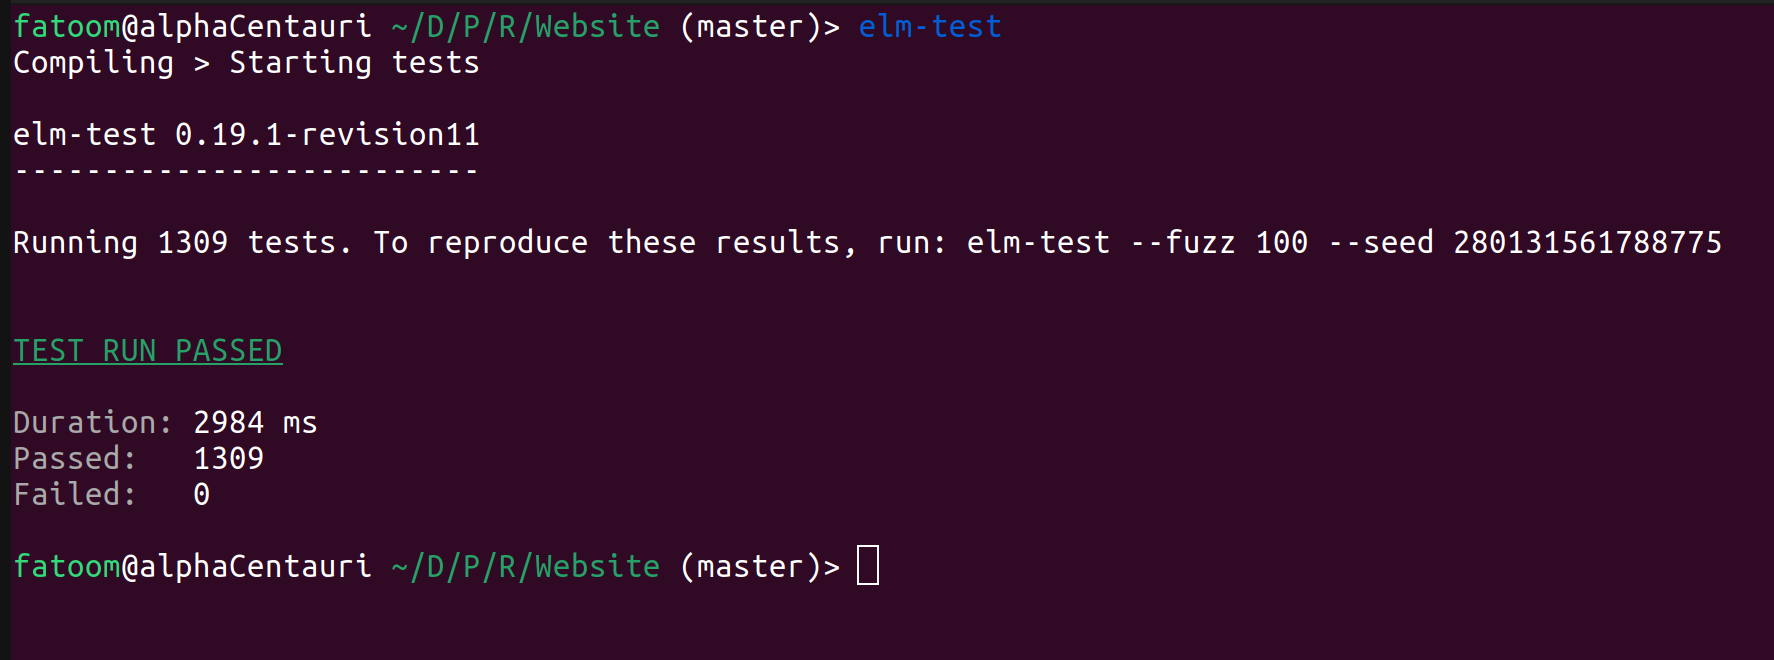
\includegraphics[width=4.70in]{testResultsSnap}
\caption{
        Results of unit and property based testing.
        }
\end{figure}

\section{Examples of Property Based Testing}
\label{testing: pbtExamples}
The first example checks if a fully connected graph is constructed well by
counting the number of edges which have been formed. The second example
generalizes this to test many types of graphs. Here also the number of edges
formed is compared against the mathematical number of edges which a particular
kind of graph should have.

\begin{lstlisting}[language=elm
                  , caption={
                  Property Based Testing of construction of a fully
                  connected graph.
                  }
                  ]
fullyConnectedGraphEdgeCountSuite : Test         
fullyConnectedGraphEdgeCountSuite =
   describe "fully connected graph edge count suite " <|
   let
      polySize =
         List.range 3 100
   in
   List.map
      fullyConnectedGraphEdgeCountTest         
      polySize

fullyConnectedGraphEdgeCountTest : Int -> Test         
fullyConnectedGraphEdgeCountTest n =
   let
      size = (vec3 100 100 0)

      pos = (vec3 100 100 0)

      graph =
         makeGraph
            (PolygonFullyConnected n)
            size
            pos
            0

      noOfEdges =
         graph.edges
         |> List.length

  in
  test ("fully connected graph edge count " ++ (String.fromInt n)) <|
   \_ ->
      Expect.equal 
         (( n * ( n - 1) )//2)
         noOfEdges
\label{listing: testA}
\end{lstlisting}

\begin{lstlisting}[language=elm
                  , caption={
                  Property Based Testing of construction 
                  graphs based on their type. For example,
                  the graph with a given number of vertices
                  should have the number of edges dependent on
                  the number of vertices.
                  }
                  ]
makeGraphNoVerticesSuite : Test
makeGraphNoVerticesSuite =
   describe "Checking if correct number of vertices is made correctly " <|
      let
         polygonSizes =
            List.range 3 200

         polygonCycles =
            List.map PolygonCycle polygonSizes

         fullyConnecteds =
            List.map PolygonFullyConnected polygonSizes

         dolls =
            List.map PolygonCycleDoll polygonSizes

         combinedGtypes =
            polygonCycles ++ fullyConnecteds ++ dolls
      in
      List.map
         makeGraphNoOfVerticesTest combinedGtypes

makeGraphNoOfVerticesTest : Gtype -> Test
makeGraphNoOfVerticesTest gtype =
      let
         sizeOfGraph =
            (vec3 150 150 0)

         positionOfGraph =
            (vec3 150 150 0)

         graph =
            makeGraph gtype positionOfGraph sizeOfGraph 0

         (expNoVer, gtypeStr) =
            case gtype of
               PolygonCycle n ->
                  (n, "Cycle")
               PolygonFullyConnected n ->
                  (n, "Fully Connected")
               PolygonCycleDoll n ->
                  (2*n, "Doll")
      in
      test 
         ("No. of vertices according to type of graph " 
            ++ String.fromInt expNoVer
            ++ gtypeStr)  <|
         \_ ->
            graph
            |> .vertices
            |> List.length
            |> Expect.equal expNoVer
\label{listing: testB}
\end{lstlisting}
